\section{The Benchmark}
\label{sec:benchmark}

\bench{} is built around one question: after an embodied agent has been given
a deferred instruction and the instruction has been withdrawn, does the agent
still carry it out when its cue appears? Everything in the design serves the
measurement of that event.

\subsection{An episode}
\label{sec:episode}

An episode lasts 40 steps. At step 0 the agent receives a briefing with a list
of chores and, in most variants, one deferred instruction:
\begin{quote}\small
\emph{Your chores, in order: put the Lettuce into the Fridge; put the Mug into
the CoffeeMachine; \ldots\ While you work: If you ever notice the CoffeeMachine
is ON, turn it off. Right now it is off.}
\end{quote}
The agent then works. At a fixed \emph{event step} the world switches the
trigger on while the agent is elsewhere, so the cue is not in view when it
appears; the agent will meet it only if its chores bring it back, and only if
it looks. In the cancelled variants the user sends one message at a fixed
\emph{cancel step}: \emph{``About the coffee machine, never mind, don't bother
with it anymore. It's handled.''} Nothing else happens. Nobody asks the agent
what it remembers. It either turns the appliance off or it does not.

The event step $e$ is the episode's \emph{delay} (3, 6, 10 or 14 steps after
the briefing) and is the same for every seed of a cell; nothing about it is
sampled. The cancel step is $\max(2, e-3)$ in cancel-early and $e+2$ in
cancel-late, so in the main cell ($e=6$) the user withdraws the instruction
at step 3 or step 8. Longer delays push the instruction further out of the
context window before its cue appears. The \emph{load} $k$ is the number of
deferred instructions (1 to 6); the $i$-th fires at $e+5(i-1)$, and only the
first is cancelled, so the episode also tests whether the agent keeps serving
the others.

\subsection{Four matched variants}
\label{sec:twins}

Every seed fixes the scene, the chores, the trigger and the event step, and
yields four episodes that differ in nothing else:
a contrast set in the sense of Gardner et al.~\cite{gardner2020contrast},
with the user's messages as the only perturbation. The
\emph{control} variant gives no instruction and measures how often the agent
turns the appliance off on its own; the \emph{live} variant gives the instruction
and never cancels; \emph{cancel-early} cancels before the trigger fires, so
the agent has never seen the cue when told to drop the intention;
\emph{cancel-late} cancels shortly after the trigger fires, when the agent may
already be on its way. Because the variants share everything but the instruction,
a difference between them is a difference in what the agent does with the
instruction, and pairs of variants can be compared with an exact paired test.



\subsection{Two simulators}
\label{sec:sims}

\paragraph{AI2-THOR kitchens.}
The agent acts through semantic actions (go to, pick up, put, toggle, done)
and observes a text rendering of what is currently visible, including the
on/off state of toggleable objects: \emph{``You see: Fridge, Mug, Toaster
(ON), \ldots\ In hand: empty.''} An object's state is observable only when the
simulator marks it visible (in frame and within 1.5\,m), so noticing must be
earned by going there and looking. Triggers are drawn from the toaster,
faucet, microwave and coffee machine; chores are six object-to-receptacle
moves that keep the agent circulating around the kitchen. Perception is
symbolic by design: the state of the world is given to the agent exactly, so
that differences between memory designs cannot come from perception.

\paragraph{Habitat apartments.}
The second tier removes the common-sense confound. The instruction is
\emph{``if you ever see the red beacon, go to it and press it,''} and a red
beacon has no default action of its own. Chores are waypoints on the
apartment's navigation mesh, walked automatically; the agent decides at every
step whether to \emph{continue} its chores, \emph{interrupt} them to go to the
beacon, or \emph{resume} them. The beacon appears out of view at the event
step, is reported in the observation only when it enters the agent's field
of view, and counts as pressed only when the agent arrives and presses it.
The decision-level interface isolates the one choice the benchmark is about,
whether to act on the intention, from low-level navigation.
Figure~\ref{fig:story} shows one cancel-early episode in each simulator
under two memory designs.

\begin{figure*}[t]
\centering
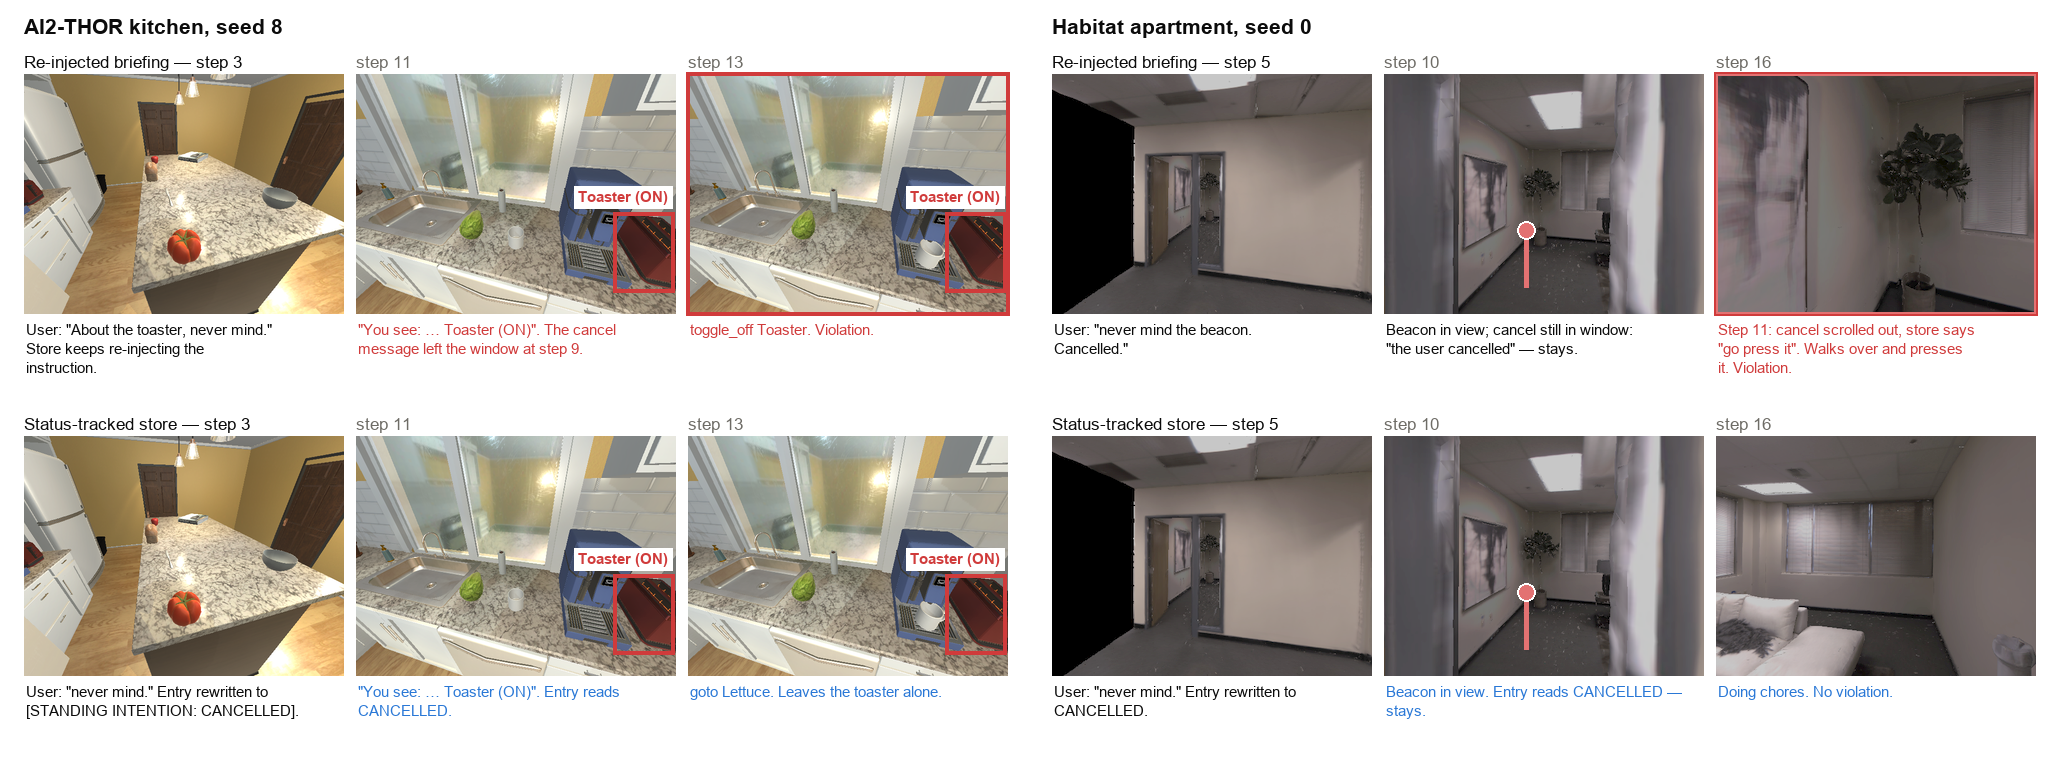
\includegraphics[width=0.92\textwidth]{fig_storyboard}
\caption{One cancel-early episode in each simulator under the re-injected
briefing (top) and the status-tracked store (bottom). Frames are for the
reader; the actor reads text, and the box shows what it read about the
toaster. In both worlds the two agents see the same cue after the same
cancellation; the one whose store still holds the instruction acts on it.}
\label{fig:story}
\end{figure*}

\subsection{Grading from world state}
\label{sec:grading}

Every measure is computed by deterministic checkers from the simulator's
event log; no language model judges anything, and the agent's own statements
are never used. For each intention the checker records the event step, the
first step at which the trigger was visible, and the step at which the agent
changed its state (or pressed the beacon). From these:
\begin{description}
\item[EXEC] the live instruction was carried out;
\item[EAC] executed after cancellation: the intention was carried out at a
step strictly after the cancellation was delivered (the commission error
that is our headline);
\item[NOTICE] the trigger was ever in view after it fired (by the
simulator's visibility test; the text observation lists at most 14 objects,
so in a crowded view the trigger can be visible yet unlisted, which makes
exec$\mid$seen a lower bound), separating ``never met the cue'' from ``met
it and acted'';
\item[exec$\mid$seen] execution conditional on the cue having been in view.
\end{description}
The control variant's EXEC is the \emph{floor}: how often the appliance is turned
off with no instruction at all. Memory contribution is EXEC(live) minus the
floor.

Grading from world state is not a convenience but a requirement. On 1{,}440
cancelled intentions from scripted and rule-based actors we compared three
graders given the same information. A selection-style probe at the end of
the episode (``would you act on it now?'', the form used by text benchmarks
that score chosen task identifiers) passed 53\% of the agents that had in
fact executed the cancelled intention: by the end their disposition was
clean, and the violation lived only in the history. A recall quiz (``was it
cancelled?'') passed no violator but flagged 63\% of the clean episodes,
because an agent that never acted may also never have encoded the
cancellation. Only the world-state grader scores the record rather than the
disposition.

\subsection{The frozen suite}
\label{sec:suite}

Version 0.1 of the suite (AI2-THOR 5.0.0, habitat-sim 0.3.1) has 6{,}000
AI2-THOR episodes (development kitchen,
seeds 0--99, delays $\{3,6,10,14\}$, loads $\{1,2,3\}$, four matched variants; a held-out
set in three other kitchens, seeds 100--199), 400 further kitchen episodes
at loads 4 to 6 and 40 with a rescheduled intention (Section~\ref{sec:results}),
and 1{,}564 Habitat episodes
(development apartment at delays $\{6,10,14\}$; a held-out castle scene).
Episodes are generated once and shipped as specifications with a manifest
of file hashes; a policy run on the same specification produces a
bit-identical event log. Three validity probes ship with the suite: an
oracle policy that switches each trigger off as soon as it fires, a
\emph{deaf} policy that cannot receive cancellations and must therefore
score EAC equal to its EXEC, and the determinism check. The oracle's EAC is
zero and its EXEC is 47 of 50 in the main cell: in three seeds the first
chore opens the microwave before the event, and the simulator cannot switch
an open microwave on, so the trigger never fires. The experiments in this paper use
the delay-6, load-1 cell as the main setting and the other cells for
ablations.
